\documentclass[a4paper, 12pt]{article}

\usepackage[utf8]{inputenc}
\usepackage[spanish]{babel}
\usepackage{graphicx}
\usepackage{fancyhdr}
\usepackage{amssymb}
\usepackage{xcolor}
\usepackage[hidelinks]{hyperref}
\usepackage[font=small, labelfont=bf]{caption} 

\topmargin=-1cm
\oddsidemargin=0cm
\textheight=24cm
\textwidth=17cm



\begin{document}

\renewcommand{\tablename}{Tabla}
\renewcommand{\refname}{Referencias y Bibliografía}



\begin{titlepage}

\begin{minipage}{2.6cm}

\includegraphics[width=\textwidth]{fceia.pdf}
\end{minipage}
\hfill
%
\begin{minipage}{6cm}
\begin{center}
\normalsize{Universidad Nacional de Rosario\\
Facultad de Ciencias Exactas,\\
Ingeniería y Agrimensura\\
Departamento de Física -- ECEN\\}
\end{center}
\end{minipage}
\hspace{0.5cm}
\hfill
\begin{minipage}{2.6cm}

\includegraphics[width=\textwidth]{unr.pdf}
\end{minipage}


\vspace{0.5cm}

\begin{center}
\normalsize{\sc Física Computacional}\\
\vspace{0.5cm}
\Large{\bf Desarrollo del software PyReduc para reducción de imágenes astronómicas}\\


\vspace{5cm}

\normalsize
Carlos Mauricio Silva\\

\vspace*{0.5cm}
\small{Agosto de 2018}

\vspace*{3cm}

\begin{abstract}
  En este trabajo se presenta el desarrollo del software PyReduc, cuyo objetivo es reducir imágenes astronómicas en formato FITS. Se comentan los fundamentos de la reducción de imágenes y se explican las funciones del programa.
\end{abstract}

\vspace{5cm}

\normalsize

\end{center}
\end{titlepage}


\pagestyle{fancy}
\lhead{\scriptsize{Desarrollo del software PyReduc}}
\rhead{\scriptsize{C. M. Silva}}
\lfoot{\scriptsize{Física Computacional}}
\cfoot{\scriptsize{Agosto de 2018}}
\rfoot{\scriptsize{Página \thepage}}
\renewcommand{\footrulewidth}{0.6pt}

%\tableofcontents
%\newpage

\section{Introducción teórica}
\subsection{Motivación}
Si hay una ciencia en la que cualquier ciudadano sin formación académica de grado puede hacer una contribución con un mínimo de equipamiento, esta es la Astronomía. Con la popularización de las cámaras ``DSLR'' (cámara digital réflex de una sola lente), cualquier persona con un poco de tiempo puede aprender laa técnicaa de astrometría y fotometría. Organizaciones como la Unión Astronómica Internacional (IAU) o la Asociación Americana de Observadores de Estrellas Variables (AAVSO) reciben las contribuciones de los observadores amateurs de todo el mundo, a quienes a través de diversas campañas se les ha comenzado a llamar ``científicos ciudadanos'' \cite{aavso}.


Si bien en Internet se puede encontrar software gratuito y de  alta calidad para realizar toda la tarea de procesado de imágenes astronómicas, estos están pensados principalmente para procesamientos artísticos o no están lo suficientemente automatizados para cumplir todas las tareas de preprocesado requeridas para poder reportar información con valor científico.

El objetivo de este trabajo es describir el funcionamiento del software \textbf{PyReduc}, desarrollado bajo las siguientes directivas:
\begin{itemize}
\item Cumplir con las libertades del Software Libre \cite{fsf}.
\item Constituir un conjunto de subrutinas  apto para realizar la reducción de imágenes, es decir el preprocesado necesario para obtener imágenes listas para realizar mediciones fotométricas sobre ellas.
\item Que el proceso de reducción sea, en la medida de lo posible, automático.
\item Que maneje el formato FITS, un formato de archivos estándar en investigación astronómica a nivel mundial. 
\item Que esté programado en un lenguaje de programación moderno, bien documentado y con librerías científicas de comprobada utilidad, como lo es el lenguaje Python.
\end{itemize}

\subsection{Algunos conceptos: Fotometría DSLR}
El objetivo de la fotometría es medir la intensidad de la luz que nos llega de los objetos celestes. Por ejemplo, en el caso de una estrella variable, esta información se hace relevante cuando se quiere obtener información sobre la evolución de la estrella en estudio.

El término ``DSLR''  se refiere a una clase genérica de cámaras
que es adecuada para llevar a cabo observaciones fotométricas. Recientemente, muchas cámaras
automáticas han comenzado a incorporar varias características requeridas para fotometría astronómica \cite{aavso}. 

En las cámaras DSLR, la imagen es capturada por un sensor electrónico de tipo CMOS (Semiconductor Complementario
de Oxido Metálico), sobre el que  se dispone un mosaico que filtra la luz en tres colores: rojo (R), verde (G) y azul (B). Estos mosaicos se conocen como mosaicos de Bayer.
Dependiendo del modelo y marca comercial de la cámara, estos mosaicos se pueden disponer en distintos órdenes. Así, por ejemplo, una la mayoría de las cámaras DSLR marca {\sf Canon} llevan un mosaico RGGB, lo que quiere decir que contiene dos celdas que detectan el verde, por cada celda de rojo y cada celda de azul. La estructura de estas cámaras escapa al objetivo de este trabajo, pero puede consultarse en la bibliografía \cite{aavso}.

El sensor en sí mismo está
hecho de un chip de silicio sobre el cual está grabado el circuito CMOS. El elemento sensible a los
fotones en cada píxel es un fotodiodo (o un sensor fotoeléctrico MOS). Tomemos, para orientarnos mejor, un único pixel en el sensor. Durante la exposición fotográfica, los fotones que van llegando al fotodiodo excitan electrones, los cuales se van almacenando en un capacitor originalmente descargado. Al final de la exposición, se lee la tensión en bornes del capacitor. Estas tensiones son muy pequeñas, por lo que para realizar la lectura se amplifican electrónicamente y luego un conversor analógico--digital (ADC) se encarga de convertirla en un número binario. En la fotometría DSLR se suele decir que este número está medido en ADU (Unidad Analógica--Digital). Este valor en ADU es el que se almacena en la matriz que conforma el archivo resultante.

Es interesante mencionar que, dado que los valores ADU registrados en la imagen son proporcionales a la cantidad de fotones que llegaron a cada pixel en cuestión, es un valor adecuado para tomar a la hora de hacer fotometría.



\subsection{El formato FITS}
Llamaremos a las imágenes de astros capturadas con fines científicos {\bf ``tomas científicas''} o {\bf ``lights''}. Las cámaras DSLR comerciales traen múltiples funciones. Entre ellas, hay algoritmos de balance de blancos, reducción de ruido, compensación de exposición, etcétera. La mayoría de estos algoritmos operan sobre los datos que capta el sensor y los modifican, por lo que es fundamental {\it no usarlos} para la fotometría. Todas las mejoras sobre las imágenes se deben hacer en perfecto control por parte del usuario. Es por ello que, al captar una toma científica, no se deben guardar en formato JPG. Al guardar en formato JPG, la imagen se convierte a un espacio de color llamado sRGB que es no lineal, y por lo tanto, no fotométrico.  El formato para almacenar tomas científicas sin pérdida de información es llamado
RAW. Un archivo RAW está formado, básicamente, por una matriz de números binarios. Cada elemento de la matriz contiene el valor ADU de cada pixel de la imagen. Además los archivos RAW conservan, en los {\it metadatos} de la imagen, información sobre la captura: marca y modelo de la cámara, sensibilidad ISO, velocidad de obturación, datos de la lente utilizada, si estuviera disponible, etcétera.

Dada la gran variedad de sensores CMOS y matrices Bayer, cada marca y modelo de cámara tiene su propio formato RAW. Para las diversas operaciones de medición astronómicas, se hace necesario tener un formato universal de imágenes. Es así que en el campo de la Astronomía y la Astrofísica se ha hecho extensivo el uso del formato FITS.

FITS es el acrónimo de {\it Flexible Image Transport System} (Sistema Flexible de Transporte de Imágenes). El formato FITS se empezó a desarrollar a fines de la década de 1970, con el uso de las primeras cámaras CCD, a los fines de compartir datos astronómicos entre instituciones que cooperaban entre sí. Una reseña histórica puede leerse en la bibliografía \cite{greisen}. Si bien la ``I'' en FITS significa ``Imágenes'', hoy en día sería más adecuada la palabra ``información'', ya que el formato FITS es mucho más que un formato de imagen. Como se establece en el sitio web de la Oficina de Soporte FITS de la NASA \cite{nasa}, en un archivo FITS se pueden guardar:

\begin{itemize}
  \item Arrays multidimensionales: Espectros 1D, imágenes 2D, Cubos de de datos de 3 o más dimensiones.
  \item Tablas que contengan filas y columnas de información (por ejemplo, coordenadas astrométricas).
  \item Una Cabecera con palabras clave (Header keywords) que provean información descriptiva sobre los datos.
\end{itemize}
  
  Un archivo FITS se divide, esencialmente en dos partes: La cabecera (header) y los datos (data).

\begin{figure}[!htb]
\begin{verbatim}
___________________________________________________________________
SIMPLE  =                    T / file does conform to FITS standard
BITPIX  =                   16 / number of bits per data pixel
NAXIS   =                    3 / number of data axes
NAXIS1  =                 5208 / length of data axis 1
NAXIS2  =                 3476 / length of data axis 2
NAXIS3  =                    3 / length of data axis 3
EXTEND  =                    T / FITS dataset may contain extensions
COMMENT   FITS (Flexible Image Transport System) format is defined in 'Astronomy
COMMENT   and Astrophysics', volume 376, page 359; bibcode: 2001A&A...376..359H
BZERO   =               32768. / offset data range to that of unsigned short
BSCALE  =                   1. / default scaling factor
INSTRUME= 'Canon EOS 700D'     / instrument name
DATE    = '2018-08-28T03:36:07' / UTC date that FITS file was created
DATE-OBS= '2018-04-14T01:36:33' / YYYY-MM-DDThh:mm:ss observation start, UT
XBINNING=                    1 / Camera binning mode
YBINNING=                    1 / Camera binning mode
EXPTIME =                  15. / Exposure time [s]
ISOSPEED=                1600. / ISO camera setting
BAYERPAT= 'RGGB    '           / Bayer color pattern
PROGRAM = 'Siril v0.9.9'       / Software that created this HDU
___________________________________________________________________
\end{verbatim}
\caption{Ejemplo de cabecera de un archivo FITS. Las palabras en mayúscula a la izquierda del signo {\tt =} son las palabras clave de la cabecera. El signo {\tt /} indica un comentario. \label{fig:header}}
\end{figure}

  
\paragraph{Cabecera FITS (Header)}
Es una sección del archivo FITS que contiene palabras clave que dan información sobre el archivo. Cuando se convierte una imagen RAW a un archivo FITS, es habitual que los {\it metadatos} de la imagen se guarden en la cabecera. También durante el procesado, esta información se va ampliando. Por tradición, la cabecera de los archivos FITS está codificada en caracteres de 7 bits ASCII.



Un ejemplo de cabecera FITS se muestra en la Figura~\ref{fig:header}.

No se presentará en este trabajo una descripción exhaustiva de las palabras claves obligatorias y opcionales que puede tener la cabecera de una archivo FITS. En cambio, se comentarán las más relevantes a los fines de este trabajo. Para más detalles, se puede consultar el manual del Estándar FITS de la Unión Astronómica Internacional \cite{fits}.

\begin{enumerate}
\item {\tt BITPIX}: Indica el número de bits por pixel (o elemento de matriz) en la sección de datos.
\item {\tt NAXIS}: Cantidad de ejes de datos. Se puede pensar como la dimensión de la matriz o el cubo de datos. En el ejemplo de la Figura~\ref{fig:header}, {\tt NAXIS1} y {\tt NAXIS2} corresponden a los dos ejes de la imagen, mientras que {\tt NAXIS3} corresponde a la cantidad de capas de color. Así podríamos decir que la imagen referenciada en el ejemplo tiene $5208 \times 3476$ pixeles y tres capas de color. La imagen de este ejemplo ya fue separada en los tres colores de los filtros del sensor. Las imágenes RAW que provienen de cámaras DSLR, deben ser separadas en colores de acuerdo con la organización del mosaico Bayer. Este proceso de descomposición se conoce como {\bf debayerizado} (debayering) o {\bf desmosaicado} (demosaicing). Si {\tt NAXIS} vale n, entonces deberán estar, necesariamente, las palabras claves {\tt NAXIS1}, {\tt NAXIS2}, ..., {\tt NAXISn}.
\item {\tt INSTRUME}: Indica marca y modelo del instrumento utilizado. Se obtiene, habitualmente, de los metadatos de la imagen RAW.
\item {\tt BAYERPAT}: Indica el patrón del mosaico Bayer de la cámara. No suele estar en los metadatos de la imagen RAW, así que al convertir el archivo a FITS se suministra esa información desde una base de datos de modelos de cámaras.
\item {\tt EXPTIME}: Es el tiempo de exposición de la imagen, medido en segundos. Equivale al tiempo que el obturador permanece abierto en una cámara convencional. En fotografía astronómica artística estos tiempos de exposición suelen ser de varias horas. A los fines de la fotometría, no es necesario tanto tiempo de exposición, fundamentalmente si se tiene en cuenta que la cámara tiene una respuesta lineal en un cierto rango de ADU. Cuando los tiempos de exposición son muy largos, puede suceder que el objeto de interés esté {\it sobreexpuesto}. En ese caso, el valor ADU registrado no será un valor proporcional a la cantidad de fotones captados por el sensor. Luego, para elegir el tiempo de exposición, un factor clave a tener en cuenta es la {\it curva de linealidad} del sensor.
\item {\tt ISOSPEED}: Es la configuración ISO en la que fue tomada la imagen. Muchas veces se dice que la configuración ISO se relaciona con la ``sensibilidad'' del sensor, pero en realidad la sensibilidad no cambia al cambiar el ajuste ISO. Lo que verdaderamente cambia con esta configuración es la {\bf ganancia} del sensor. La  ganancia se suele medir en electrones por ADU ($e^{-}$/ADU), y es una medida de la amplificación de la señal.
  Cuando un fotón llega al sensor, existe siempre la misma probabilidad de que este excite un electrón produciendo una señal. Esta respuesta a la excitación sería la sensibilidad del sensor. La ganancia, en cambio, está caracterizada por la amplificación de la señal producida. Configuraciones ISO más altas dan una ganancia más pequeña. Esto significa que para obtener una unidad ADU, a ISO más alto, se necesitará excitar menos electrones. Resumiendo, podemos decir que a mayor ISO, mayor amplificación de la señal, y menor ganancia. Un problema que surge al aumentar la configuración ISO es que también aumenta el ruido. Es por ello que, para fotografía astronómica no se usan las configuraciones ISO más altas. En fotografía astronómica artística, las configuraciones ISO suelen estar entre ISO 800 y 3200. En cambio, para las técnicas de fotometría, se busca que la ganancia del sensor sea cercana a 1 $e^{-}$/ADU. Como ejemplo, en la DSLR {\sf Canon EOS 700D}, esto se logra para ISO 200 o ISO 400. %En el Apéndice~\ref{ap:gain} se presentan gráficas de la ganancia del sensor para estas dos configuraciones.
\item {\tt DATE}: Es la fecha y hora de creación del archivo FITS.
\item {\tt DATE-OBS}: Es la fecha y hora en que se realizó la toma%\footnote{Como este informe, que fue escrito durante la toma de la FCEIA.}
  fotográfica, en {\it Tiempo Universal Coordinado}. Este valor se obtiene de los metadatos de la imagen, que a su vez se obtienen de la configuración de la cámara. Para esto, es importante que la hora de la cámara esté bien sincronizada con la hora oficial.

  Como decíamos, otras palabras claves son posibles, como la ubicación geográfica del observatorio, el nombre del observador, el nombre del objeto observado, sus coordenadas celestes, etcétera.
\end{enumerate}

\paragraph{Datos FITS}
Son los datos propiamente dichos, codificados en binario según la palabra clave {\tt BITPIX}, y ordenados en un arreglo de dimensiones indicadas por las palabras claves {\tt NAXIS1}, {\tt NAXIS2}, ..., {\tt NAXISn} de la cabecera. Con estos datos se trabajará en la reducción de imágenes y la fotometría.


\subsection{Reducción de imágenes: Tomas Dark, Bias y Flat}
\label{sec:tomas}
El proceso de reducción implica la eliminación de efectos instrumentales que estén presentes en los datos, ya sean de espectroscopía o de imagen directa. Es necesario llevar a cabo la reducción antes de poder realizar cualquier tipo de medida sobre nuestros datos. En este trabajo nos limitaremos a los efectos comúnmente presentes en las imágenes DSLR, pero esencialmente estos son los mismos efectos que se presentan en las imágenes con sensores CCD.

Podríamos decir que el mayor problema con el que hay que lidiar en la fotometría DSLR es con el ruido. Dado que en la fotometría necesitamos relevar la intensidad de la luz que proviene de las estrellas, necesitamos que el ruido sea lo sufientemente bajo para que no interfiera significativamente con las mediciones. Es por ello que el objetivo principal que se persigue con el proceso de reducción es incrementar la {\bf ``relación señal/ruido''} (SNR).

\subsubsection{Tomas Bias}
\label{sec:bias}
Al igual que en las tomas Dark, las tomas Bias se realizan con el objetivo tapado, y la misma configuración ISO que las tomas científicas, pero con la exposición más corta que proporcione la cámara (por ejemplo, 1/4000 s). Estas tomas contienen el ruido electrónico y de lectura propio del sensor. Este ruido está presente en todas las tomas, independientemente de la exposición y de la temperatura del sensor. Con el conjunto de tomas Bias se realiza un apilado promediando los valores de los pixeles homólogos de cada imagen, o bien tomando la mediana de dichos valores. Al hacer esto se crea un \textbf{``Master Bias''}.

\subsubsection{Tomas Dark}
Una de las correcciones que se pueden hacer a nuestras tomas científicas es la corrección por tomas Dark. Las tomas Dark se realizan con la misma configuración ISO que las tomas científicas y la misma exposición, pero ``en la oscuridad''. Para ello, se tapa el objetivo de la cámara o del telescopio y se dispara una serie de tomas, usualmente más de diez. Las tomas Dark, entonces, no contienen ``información'', pero contienen ruido térmico asociado con el sensor. Este ruido térmico es fuertemente dependiente de la temperatura y de la exposición. Así, para exposiciones menores a 30 s, pueden no ser necesarias estas tomas de calibración. Sin embargo, para exposiciones prolongadas, el sensor va aumentando su temperatura y el ruido térmico se hace más evidente. También la temperatura ambiente juega un rol fundamental en esta ecuación. Es por ello que las tomas Dark deben hacerse durante la misma sesión fotográfica, aunque eso quite tiempo de exposición para las tomas científicas.

\begin{figure}[!ht]
  \centering
  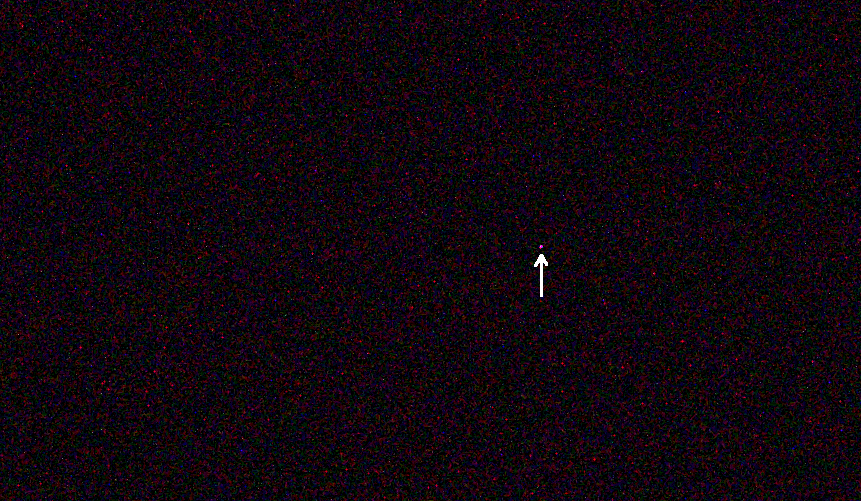
\includegraphics[width=0.75\textwidth]{img/dark.png}
  \caption{\label{fig:dark} Recorte y ampliación de una toma Dark realizada con una DSLR Canon EOS 700D en un telescopio Maksutov-Cassegrain de 102 mm f/12,7. La imagen RAW está debayerizada y el contraste está levemente realzado. La flecha blanca muestra un defecto que no vuelve a aparecer en el resto de imágenes Dark de la serie y se puede deber, por ejemplo, al efecto de rayos cósmicos impactando en el sensor. Si este efecto apareciera en toda la serie de imágenes, entonces podríamos decir que es un defecto de lectura del sensor, conocido como ``hot pixel''.}
\end{figure}

Con el conjunto de tomas Dark, usualmente se hace un apilado promediando los valores de los pixeles homólogos de cada imagen, o bien tomando la mediana de dichos valores.  Sin embargo, como se decía en la sección \ref{sec:bias}, estas tomas también tendrán ruido electrónico y de lectura. Para quitar esta contribución, se le puede restar a cada toma Dark un Master Bias. Este último proceso es especialmente importante si las tomas Dark no tienen el mismo tiempo de exposición que las tomas científicas. Finalmente se deben apilar las imágenes Dark corregidas utilizando el promedio o la mediana de los pixeles, obteniendo así una imagen que se llama \textbf{``Dark-current''}. Antes de restar la imagen Dark-current a las tomas científicas, se las debe escalar por un factor igual al cociente entre el tiempo de exposición de las tomas científicas y de las tomas Dark.

\subsubsection{Tomas Flat}
Los telescopios y las lentes comerciales usualmente no iluminan el sensor en forma homogénea. Habitualmente, la luz se distribuye en mayor cantidad en el centro del sensor que en los bordes. Este defecto en las imágenes se llama viñeteo. Más aún, las superficies ópticas de los telescopios y lentes suelen acumular polvo (y el sensor de la cámara también). A esto hay que agregarle que el propio sensor no tiene la misma respuesta en todos sus pixeles a un mismo estímulo lumínico. 
La Figura~\ref{fig:flat} muestra una toma flat individual con el contraste realzado para mostrar algunos defectos que se pueden presentar en una imagen. A diferencia de los ruidos térmico y de lectura, que eran contribuciones aditivas a las tomas científicas, estos defectos son de carácter multiplicativo. Para corregir estos defectos, se debe dividir a las tomas científicas por un {\bf ``Master Flat''}.

\begin{figure}[!ht]
  \centering
  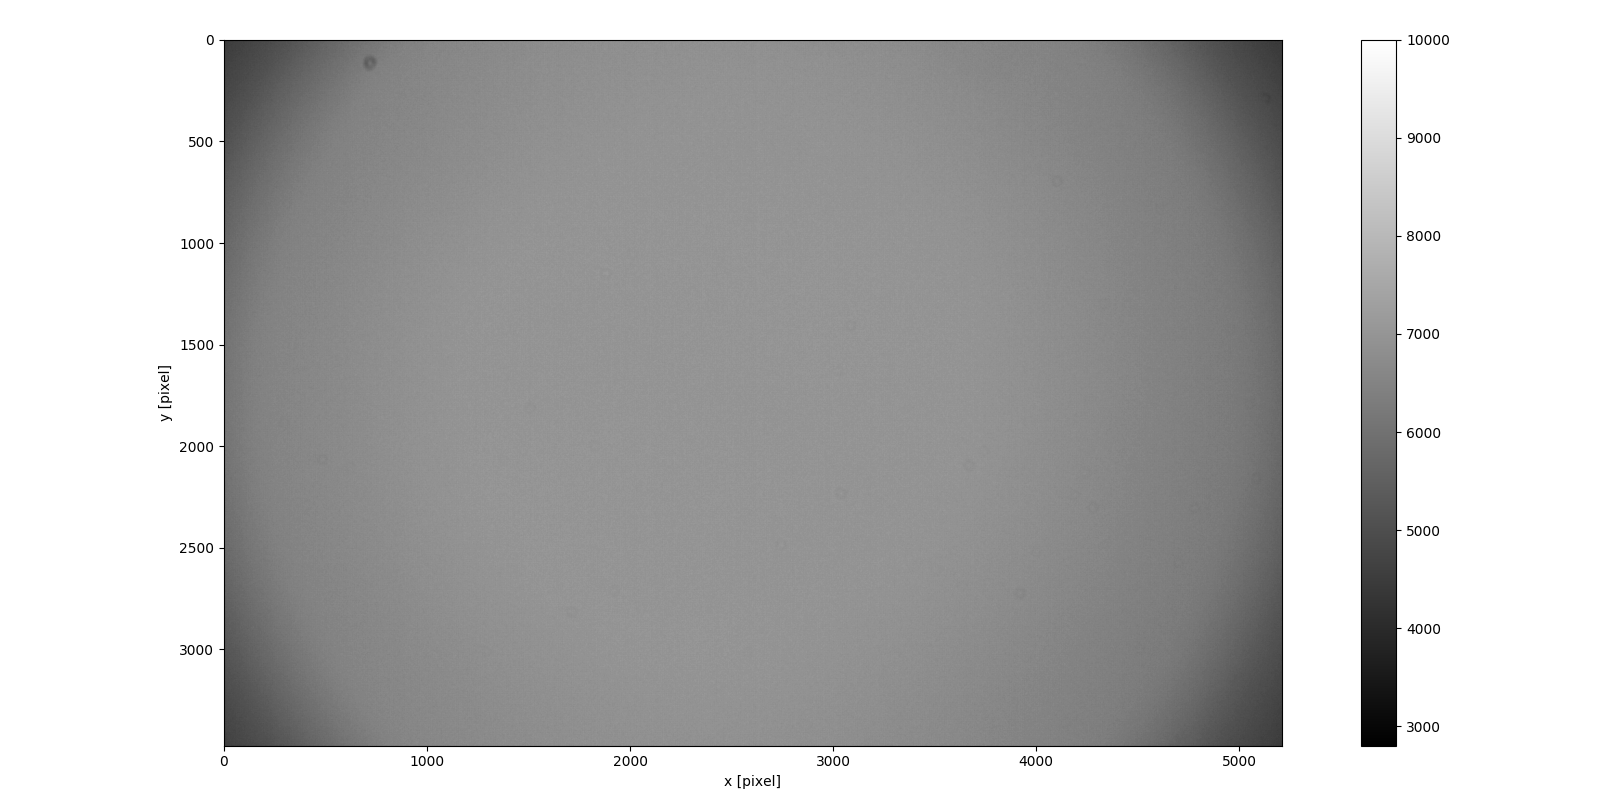
\includegraphics[width=\textwidth]{img/flatx.png}
  \caption{\label{fig:flat} Toma Flat realizada con una DSLR Canon EOS 700D en un telescopio Maksutov-Cassegrain de 102 mm f/12,7. Se muestra solo el canal verde de la imagen. Se observa en las esquinas de la imagen el efecto de viñeteo debido a una iluminación no homogénea del sensor. También arriba a la izquierda de la imagen se ve una mancha circular que se debe a un resto de polvo en el tren óptico del instrumento.}
\end{figure}

Para fabricar un Master Flat, se deben sacar varias tomas apuntando el objetivo a una superficie uniformemente iluminada por luz blanca, sin llegar a saturar el sensor. Una manera simple y moderna de hacerlo es apuntar el telescopio a un monitor LCD (sin remover la cámara de su posición en el tubo). Las cámaras DSLR comerciales tienen un modo AV en el que la cámara calcula el tiempo de exposición automáticamente. Este modo usualmente proporciona Flats muy adecuados. La configuración ISO en el caso de las tomas Flats debe ser menor o igual a la de las tomas científicas.

Una vez que se tienen las tomas Flat, se les debe quitar el ruido de lectura y térmico restándole los Master Bias y Dark-current (escalado con el tiempo de exposición de los Flats). Luego se las apila utilizando la mediana, siendo el resultado obtenido el Master Flat. Antes de dividir las tomas científicas por el Master Flat, se le debe realizar un escalado o normalización, ya que es posible que los niveles de iluminación sean diferentes para cada imagen. Una opción posible sería darle peso a cada imagen Flat usando su mediana. Se promedian todas las imagenes Flats utilizando esos pesos, y se divide esta imagen resultante por el promedio de todos sus pixeles. La imagen Master Flat resultante está, entonces, reducida y normalizada.


Las correcciones explicadas en toda esta sección \ref{sec:tomas} se pueden condensar en la fórmula~(\ref{eq:reduc}).


\begin{equation}
  \mbox{Científicas}_{reducidas} = \frac{\mbox{Científicas}_{raw} - \mbox{Master~Bias}-\mbox{Dark~current}_{escalada}}{\mbox{Master~Flat}_{reducida,~normalizada}}
  \label{eq:reduc}
\end{equation}

 Esta fórmula de reducción de imágenes científicas que se utiliza aquí fue tomada del curso
 ``Introduction to Astronomical Image Analysis'' de  Matthew Craig, Juan Cabanela y Linda Winkler \cite{craig}.

Una vez que la serie de imágenes científicas fueron reducidas, se puede proceder a realizar las mediciones fotométricas. Sin embargo, si se busca realizar una medición precisa de un objeto muy débil, se puede aumentar aún más la SNR. Esto se logra realizando un apilado (en inglés \textit{stacking}) de un conjunto de tomas científicas reducidas de la misma región del cielo. Para este apilado existen diferentes algoritmos. El más sencillo consiste en promediar los pixeles homólogos de cada imagen, como se hacía con las tomas de calibración. Otros algoritmos consisten en realizar ese promedio, pero descartando valores extremos o reemplazándolos por valores que  se encuentren dentro de ciertos percentiles.

Como último detalle, puede que la serie de imágenes no estén perfectamente alineadas, por ejemplo, porque el seguimiento del telescopio utilizado no es perfecto. Es por ello que muchas veces se hace necesario hacer una alineación, llevando todas las imágenes de la serie a un mismo sistema de coordenadas mediante traslaciones, rotaciones y, en casos más raros en que se usen distintas lentes, cambios de tamaño. Este proceso se llama {\bf ``Registro de imágenes''} \cite{brown}.

\section{Metodología}
Para desarrollar el programa PyReduc se ha utilizado el lenguaje de programación Python 3. Este lenguaje de alto nivel, interpretado y orientado a objetos, posee una gran variedad de librerías científicas. Entre ellas, la librería \texttt{NumPy} es fundamental para trabajar con vectores, matrices y arreglos N-dimensionales. Integrado dentro de la gran librería \texttt{SciPy}, \texttt{Matplotlib} permite graficar \textit{al vuelo} funciones, datos o imágenes de mapas de bits. Por otro lado, la librería \texttt{Astropy} es un esfuerzo comunitario por desarrollar todo un ecosistema de paquetes astronómicos que sean interoperables en lenguaje Python \cite{astropy}. Entre ellos, el módulo \texttt{astropy.io.fits} permite manejar ficheros FITS. Está basado en el módulo \texttt{PyFITS} desarrollado por el Space Telescope Science Institute. El proyecto \texttt{PyFITS} se unió a \texttt{Astropy} como parte de estos esfuerzos de desarrollar una gran librería--ecosistema de paquetes astronómicos.

Dado que PyReduc está pensado para realizar reducciones que luego se utilizarán para fotometrías, el programa está pensado para procesar  imágenes FITS monocromáticas. En el caso de imágenes RAW DSLR, será necesario, antes de utilizar PyReduc, realizar el debayerizado y extraer un canal con algún software externo. Una posibilidad sería utilizar el script de M. Emre Aydin \texttt{cr2fits} \cite{aydin}, que permite extraer un solo canal de una imagen RAW y la convierte en FITS, transcribiendo todos los metadatos necesarios.

Las imágenes FITS deben estar en un directorio llamado ``\texttt{\~/pyreduc/FITS/}'',  donde ``\texttt{\~}'' representa el directorio \texttt{HOME}. Los prefijos de los archivos deben seguir las siguientes reglas:
\begin{itemize}
\item[--]  FLATS: ``\texttt{flat*}''
\item[--]  DARKS: ``\texttt{dark*}''
\item[--]  BIAS: ``\texttt{bias*}''
\end{itemize}
donde ``*'' significa ``cualquier cosa a partir de aquí''.
El prefijo de las tomas científicas se ingresa por teclado.

Por ejemplo:\\

 En la carpeta ``\texttt{\~/pyreduc/FITS/}'' se tienen los archivos:
\begin{verbatim}
  - bias001.fit, bias002.fit, bias003.fit bias004.fit,...
  - darkA.fit, darkB.fit, darkC.fit,...
  - flat_0001.fit,..., flat_0005.fit,..., flat_0011.fit
  - RCnc_001.fit, RCnc_002.fit, RCnc_003.fit,...,
\end{verbatim}
 entonces las tomas de calibración tienen el nombre correcto. Cuando el programa pida el prefijo de las tomas científicas,
se deberá ingresar por teclado:
\begin{verbatim}
	RCnc
\end{verbatim}





Una vez que todos los archivos FITS de tomas científicas, Flats, Dark y Bias están dispuestas en una carpeta FITS dentro del directorio \texttt{\~/pyreduc/FITS/}, PyReduc las copia, utilizando la librería \texttt{shutil}, a un nuevo directorio llamado ``\texttt{\~/pyreduc/procesado/}'', en el que se realizará el proceso de reducción.

Utilizando la librería \texttt{glob}, se arman 4 objetos de tipo {\em lista} de Python 3, que contendrán las tomas científicas, dark, bias y flat. Luego, empleando la librería {\tt astropy.io.fits} se leen las cabeceras de estos archivos y se imprimen por pantalla los nombres de archivos junto con la resolución en pixeles de cada imágen y el tiempo de exposición.

La cantidad de archivos de cada lista se guarda en una variable distinta. Además se guardan en sendas variables el tiempo de exposición de cada tipo de toma. En este punto, hay que destacar que en PyReduc suponemos que todas las tomas de un mismo tipo tienen el mismo tiempo de exposición, por lo que puede que alguna parte del proceso no se cumpla si esta suposición no es verdadera.

Una vez hecho esto, comienza el proceso de reducción propiamente dicho. Este proceso está basado en un trabajo de Ricardo Gil-Hutton \cite{gil-hutton}. Este tutorial estaba basado en la librería \texttt{PyFits},
pero en PyReduc se ha  reemplazado por {\tt astropy.io.fits}.


 Para realizar el procesado de Bias se sigue el método descripto a continuación:
 \begin{enumerate}
 \item Primero se arma un arreglo tridimensional en donde se ponen todas las imágenes Bias secuencialmente, de manera que el elemento $a_{ijk}$ del arreglo es el pixel de coordenadas $(j,k)$ de la {\it i-ésima} imagen Bias.
 \item Luego se ordenan los pixeles de la secuencia de imágenes de menor a mayor a lo largo del primer eje. Para clarificar esto, se toman los pixeles de coordenadas fijas $(j,k)$ de cada imagen de la secuencia y se los ordena de mayor a menor en el arreglo tridimensional. Así, la matriz que se obtendría de fijar el índice $i=0$\footnote{A diferencia del lenguaje FORTRAN, en el lenguaje Python los índices de los arreglos comienzan en 0.} estaría formada por los pixeles de menor valor de todas las imágenes. Este ordenamiento se realiza con la función \texttt{sort} de la librería \texttt{NumPy}.
 \item Finalmente se calcula la mediana de todos los pixeles de coordenadas $(i,j)$ fijas, pero descartando los pixeles de valor más alto. Este cálculo de la mediana se realiza con la función \texttt{median} de la librería \texttt{NumPy}.
 \end{enumerate}
 

 La imagen así obtenida constituye el Master Bias, el cual se guarda en memoria, en un array de \texttt{NumPy} de nombre \texttt{stbias}. A continuación, se sigue con el procesado de tomas Dark. Lo primero que se hace es restarle a todas las tomas Dark el Master Bias, formando así tomas pre-Dark-current. Para este fin, se creó una función llamada \texttt{resta\_master} cuyos argumentos son la lista de imágenes a procesar y la imagen Master que se les va a restar. Cabe destacar que esta función sobreescribe las imágenes de la lista que se le pasa como argumento, reemplazándolas por las nuevas imágenes pre-Dark-current.

 Una vez que se tienen las imágenes pre-Dark-current, se realiza el procedimiento de obtención de la mediana 

 



   

\begin{thebibliography}{100}
\bibitem{aavso} American Association of Variable Star Observers: {\it ``Manual de Observación DSLR de AAVSO''}, Versión 1.1 en Español, 2015. En Internet: \url{https://www.aavso.org/dslr-observing-manual}
  \bibitem{fsf} Free Software Foundation: {``Qué es el software libre?''}, Versión 1.153, 2017. En Internet: \url{https://www.gnu.org/philosophy/free-sw.es.html}
\bibitem{greisen} Eric W. Greisen: {\it ``FITS: a remarkable achievement in information exchange''}, 2003. En: Heck A. (eds) Information Handling in Astronomy - Historical Vistas. Astrophysics and Space Science Library, vol 285. Springer, Dordrecht. \url{https://doi.org/10.1007/0-306-48080-8_5}
\bibitem{phillips} Dwayne Phillips: {\it ``Image Processing in C''}, 2nd Ed, 2000. En Internet: \url{http://homepages.inf.ed.ac.uk/rbf/BOOKS/PHILLIPS/cips2ed.pdf}
\bibitem{gil-hutton} Ricardo Gil-Hutton: {\it ``Cómo hacer una reducción básica de imágenes FITS con Python''}, Noviembre 2016. En Internet: \url{https://freeshell.de/~rgh/arch/python/python-red-basica.pdf}
\bibitem{nasa} The FITS Support Office: {\it ``What is FITS?''}, NASA. Última revisión, Diciembre 2017.  En Internet: \url{https://fits.gsfc.nasa.gov/}
\bibitem{fits} FITS Working Group, International Astronomical Union: {\it ``Definition of the Flexible Image Transport System (FITS)''}, Version 4.0, 2016. En Internet: \url{https://fits.gsfc.nasa.gov/standard40/fits_standard40aa-le.pdf}
\bibitem{craig} Matthew Craig, Juan Cabanela, Linda Winkler: {\it ``Introduction to Astronomical Image Analysis''}, 2014. En Internet: \url{https://image-analysis.readthedocs.io}
\bibitem{brown} Lisa G. Brown: {\it ``Image Registration Techniques''}, ACM Computmg Surveys, Vol 24, No. 4, 1992. \url{https://doi.org/10.1145/146370.146374}
\bibitem{astropy} Astropy Collaboration: {\it ``The Astropy Project: Building an Open-science Project and Status of the v2.0 Core Package''}, The Astronomical Journal, Volume 156, Issue 3, article id. 123, 19 pp., 2018. \url{https://doi.org/10.3847/1538-3881/aabc4f}
\bibitem{aydin}  M. Emre Aydin: ``{\it cr2fits v2}'', Version v2.1.0, 2017, May 21, Zenodo. \url{http://doi.org/10.5281/zenodo.581722}
\end{thebibliography}





\appendix
%\section{Linealidad y ganancia de una cámara DSLR}
%\label{ap:gain}
%En esta sección se muestran gráficas de linealidad y ganancia para la cámara DSLR {\sf Canon EOS 700D}. No es el objetivo de este trabajo explicar cómo se lleva a cabo esta medición.

%\begin{figure}[!ht]
%  \centering
%  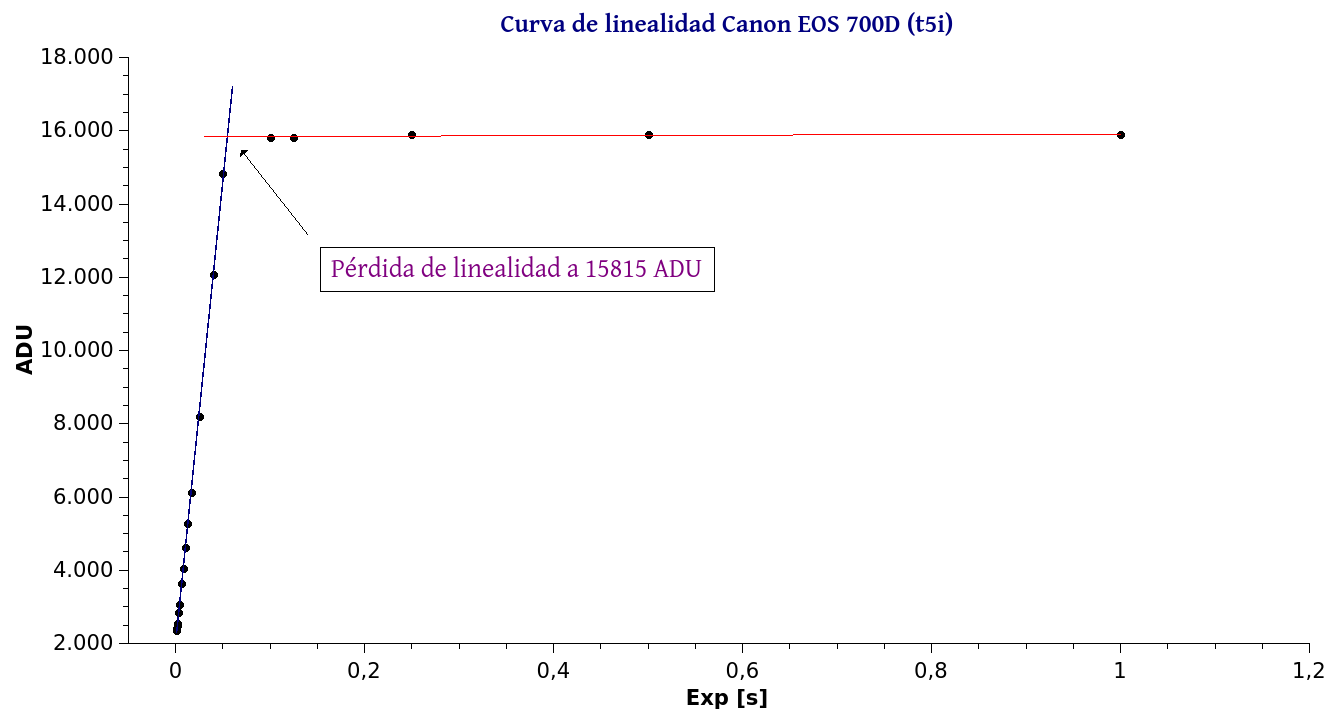
\includegraphics[width=0.8\textwidth]{img/linealidad.png}
%  \caption{\label{fig:linealidad} Curva de linealidad para la cámara DSLR {\sf Canon EOS 700D}}.
%\end{figure}


\end{document}